\newpage
\section{Introduction}
\quote{``Desar's chosen field in mathematics was so esoteric that nobody in the institute or the Maths Federative could really check his progress"
\\\textit{The Dispossessed, Ursula K. Le Guin}}
\vspace{2ex}
\subsection{Homotopy groups of spheres}
Let $(X,x_0)$ be a pointed topological space - we will often leave the basepoint implied. A major goal of algebraic topology is to study the topology of $X$ via homotopy invariants. One of the first invariants we meet are the \defn{homotopy groups} of based maps from spheres\footnote{What's so special about spheres? You'll see...} into $X$. For $n\geq 0$, these are defined as $\pi_n(X)=[S^n,X]_*=Map_*(S^n,X)/\sim$, where $f\sim g\iff$ there exists a homotopy $h:f\simeq g$. The quotient map $h:S^m\rightarrow S^m/\sim \iso S^m\wedge S^m$ that identifies the "equator" of $S^m$ with a point gives rise to a map $$\pi_n(X)\times \pi_n(X)\iso Map_*(S^n\wedge S^n,X)\rightarrow \pi_m(X)$$ by precomposition with $h$. This gives a group structure on $\pi_n(X)$ when $n\geq 1$, which is abelian when $n\geq 2$. Even more pleasantly, this construction is functorial, yielding functors $\pi_n:\text{Top}_*\rightarrow Ab$ when $n\geq 2$.

A reasonable first problem is to study the homotopy groups of spheres $\pi_n (S^m)$. When $n\leq m$, these have a satisfying structure:

\begin{theorem}{thm:easy-hom-groups-of-spheres}

Let $0<m\in \N$. Then 
$$\pi_n(S^m)\iso\begin{cases}0,&n<m\\ \Z, & m=n\end{cases}$$
\end{theorem}

The maps in $\pi_1S^1$ are classified, up to homotopy, by degree, with $d\in \Z$ corresponding to the map $s_d:S^1\rightarrow S^1 \quad z\mapsto z^d$. The isomorphisms $\pi_1(S^1)\iso \pi_n(S^n)$ can be identified via the Hurewicz homomorphism, which we will study later. It is intuitive, but not trivial, to show $\pi_n(S^m)=0$ when $n<m$. In the case $n=1,m=2$ it can be thought of as the statement "a rubber band on a ball can always be slid off". It follows from the cellular approximation thereom, which states any map $f:X\rightarrow Y$ between CW-complexes is homotopic to a cellular map, that is, one which takes the $n-$skeleta of $X$ to the $n-$skeleta of $Y$. Since $S^m$ has a CW-structure with one $0$-cell and one $m$-cell, it follows that any map $f:S^n\rightarrow S^m$ for $n<m$ is homotopic to a constant map. Lastly, let's consider the groups $\pi_n S^1$ for $n>1$. A map $X\rightarrow Y$ where $X$ is simply connected has a lift to a cover $\tilde{Y}$ of $Y$. This shows any map $f:S^n\rightarrow S^1$ where $n\geq 2$ is null-homotopic, since it factors through the universal cover of $S^1$, $\R$, which is contractible. We therefore have a full classification of $\pi_n(S^1).$

\begin{theorem}{thm:homotopy-groups-of-S1}

\[\pi_n(S^1)\iso\begin{cases}0, & n\neq 1\\ \Z, & n=1\end{cases}\]

\end{theorem}

We might hope (and expect) that the higher homotopy groups of all spheres are this simple. After all, \textit{it's just spheres} - how complicated can it be? As it turns out, very complicated. The first indication of this was found by Hopf. The CW-complex structure of $\CP{2}$ is given by adjoining a $4$-cell to $\CP{1} \simeq S^2$ in the following way: recall $\CP{2}=\C^3/\sim$ where $[x,y,z]\sim \lambda [x,y,z]$ for $\lambda \in \C$, and notice the subset given by $z\neq 0$ is homeomorphic to $\text{int}(D^4)$ via the homeomorphism $[x,y,z]= [x/z,y/z,1]\mapsto (x/z,y/z)$, while the subset given by $z=0$ is homeomorphic to $\CP{1}$. We therefore adjoin a $4-$cell via the quotient map $S^3\subset \C^2 \rightarrow \CP{1}$. This is a fibration, and the fiber over each point is given by $\{\lambda\in \C:|\lambda|=1\}\iso S^1$. This gives a fibration
$$S^1\rightarrow S^3\rightarrow S^2$$
called the \defn{Hopf fibration}. The corresponding long exact sequence in homotopy reads
$$\dots\rightarrow \pi_3(S^1)\rightarrow \pi_3(S^3)\rightarrow \pi_3(S^2)\rightarrow \pi_2(S^1)\rightarrow \dots$$
so by our previous calculations we have $\pi_3(S^2)\iso \Z$! 

In some sense, the nontriviality of higher homotopy groups of spheres comes from the failure of the suspension functor $\Omega:Top_*\rightarrow Top_*$ to be an equivalence. If it were an equivalence, we would have $\Omega S^n\simeq S^{n-1}$ and the loop space fibration $\Omega S^n\rightarrow PS^n\rightarrow S^n$, where $PX$ are the space of paths in $X$, would read $S^{n-1}\rightarrow *\rightarrow S^n$ up to homotopy equivalence. The long exact sequence in homotopy would then give $\pi_k S^n\iso \pi_{k-1}S^{n-1}$ for all $k$. This desire for $\Omega$ to be an equivalence will shortly lead to some interesting maths.

Let us now compare with homology. The homology functor $H_*:Top_*\rightarrow grAb$ is in a sense a completely algebraic homotopy invariant. They are easy to compute compared to homotopy groups, thanks to the presence of \textit{excision}. A concrete form of the excision axiom says: given a pair $(X,A)$ of topological spaces, with $A\subset X$, and a subset $U\subset A$ such that $\overline{U}\subset int(A)$, the inclusion $$(X\setminus U, A\setminus U) \hookrightarrow (X,A)$$ induces an isomorphism in (reduced) relative homology. Excising a small disk $D^n$ from the pair $(S^n, D^n)$, of an $n$-sphere and its upper hemisphere, gives an isomorphism $H_n(S^n,D^n)\iso H_n(D^n,S^{n-1}).$ Combining the two long exact sequences in (reduced) relative homology gives isomorphisms $$\tilde{H}_k(S^n)\iso \tilde{H}_{k-1}(S^n,D^n)\iso \tilde{H}_{k-1}(D^n,S^{n-1})\iso \tilde{H}_{k-1}(S^{n-1}).$$ The reduced homology groups of $S^n$ are therefore the same as those of $S^1$, shifted by $n-1$ in degree. Clearly we have $$\tilde{H}_n(S^0)=\begin{cases}\Z&n=0\\ 0&\text{otherwise}\end{cases}$$ and therefore
$$H_n(S^m)=\begin{cases}\Z& n=0 \text{ or } n=m\\ 0&\text{otherwise}\end{cases}$$

The previous discussion says homology groups of spheres are stable under suspension $\Sigma: H_k(S^n)\xrightarrow{\iso} H_{k+1}(\Sigma S^n)$. Since we don't have excision for homotopy groups, we can't expect a similar result. However, it turns out that we almost have stability, in the following sense:
\begin{theorem}[The Freudenthal suspension theorem]{thm:Freudental}
The homomorphism $\sigma:\pi_{n+k}(S^n)\rightarrow \pi_{n+k+1}(S^{n+1})$ induced by suspension is an isomorphism when $n\geq k+2$.
\end{theorem}
This theorem states that the homotopy groups of spheres are \textit{eventually} stable under $\Sigma$. We have already confirmed this result for $n\leq m$, giving us the first non-trivial stable value $\pi_2S^2=\Z$. After calculating $\pi_4S^3=\Z/2\Z$ we would then have
$$\Z/2\Z\iso\pi_4S^3\iso\pi_5S^4\iso\dots$$
We denote the group $$\pi_n^s:=\pi_{2n+2}S^{n+2}=\colim_{k\in \N}\big(\pi_{n+k}(S^k)\big) \text{ for } n\geq 2$$ the $n^{\text{th}}$ \defn{stable homotopy group of spheres}.

The following table shows some of the homotopy groups of spheres, with the stable homotopy groups highlighted. Note that in some cases, stability comes earlier than promised. We notice all of the groups are finitely generated, and most of them are finite. This was proven in generality by Serre.
\begin{theorem}[Serre]{thm:Serre}
    The homotopy groups $\pi_n(S^m)$  are finite, except for
    $$\pi_n(S^n)=\Z \text{ for } n\geq 1$$
    and $$\pi_{4m-1}(S^{2m-1})=\Z\oplus A$$
    where $A$ is finite.
\end{theorem}

In particular, the stable homotopy groups are finite for $n\geq 1.$
\begin{figure}[h!]
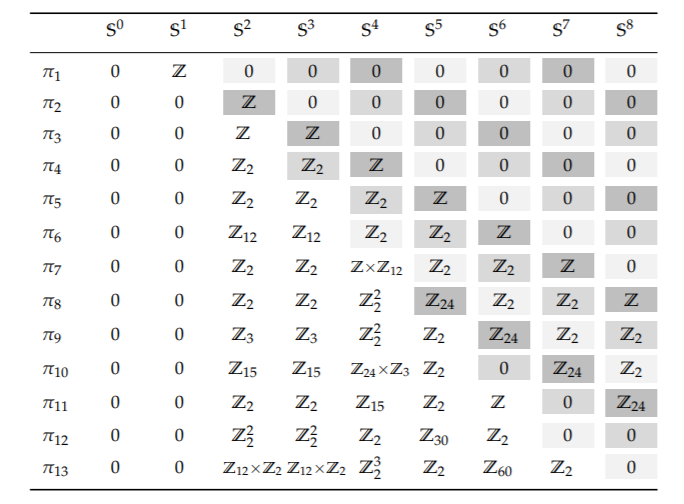
\includegraphics[width=14cm]{Content/stable.png}
\centering
\caption{Some homotopy groups of spheres, taken from the HoTT book, \cite{HoTT}.}
\end{figure}

\subsection{Homology theories}
Let us cast an old story in a new light. 
\begin{definition}{def:homology-functor}A \defn{(reduced) homology functor} is a functor
$$\tilde{E}_*:HoS_*\rightarrow grAb$$
from the homotopy category of pointed spaces to the category graded abelian groups, along with a natural suspension ismorphism $$\sigma:\tilde{E}_*\rightarrow \tilde{E}_{*+1}\circ \Sigma,$$ such that
\begin{enumerate}[(i)]
\item (Finitary) $\tilde{E}_*$ preserves filtered colimits.
\item (Excisive) Given an inclusion $A\xhookrightarrow{} X$ we obtain an exact sequence $$\tilde{E}_*(A)\rightarrow \tilde{E}_*(X)\rightarrow \tilde{E}_*(X/A).$$
\end{enumerate}
\end{definition}

%\begin{remark}

We can compare this definition to the classical one by Eilenberg and Maclane (...)
%\end{remark}

The long exact sequence in homology comes straight from the definition by consecutively taking homotopy quotients:
% https://tikzcd.yichuanshen.de/#N4Igdg9gJgpgziAXAbVABwnAlgFyxMJZABgBpiBdUkANwEMAbAVxiRAEEQBfU9TXfIRQBGclVqMWbABrdeIDNjwEio4ePrNWiENID0nHnyWCiZddU1SdAKjnGBKlACYxlydpB2jC-sqHIrhYSWmwAOmEAylgA5gC2dAAEhvKKjgGuzhoe4VGxCYmyPmn+qqRZ7qG29r4mTsgAzOXZVSAR0fF0ABT67ACUNSWmKE3BVp7eqX7DgaQNLdZtYVAQOAhc4jBQMfBEoABmAE4QcUhkIDgQSMI+Rydn1JdIDbfHp4hNF1eIzq-3iKIvkhfvI7u9AU9EAAWP7vVxAxAAVlhSChj2+yNBb2B6KQAHYUYg8bjEAA2QmIknkrH-SkIgCchPpJIAHITSaz2SThMQNlwgA
\[\begin{tikzcd}
A \arrow[r] \arrow[d] & X \arrow[d] \arrow[r]   & * \arrow[d]                  &             \\
* \arrow[r]           & X/A \arrow[r] \arrow[d] & \Sigma A \arrow[d] \arrow[r] & * \arrow[d] \\
                      & * \arrow[r]             & \Sigma X \arrow[r] \arrow[d] & \Sigma(X/A) \\
                      &                         & \dots                        &            
\end{tikzcd}\]
This gives rise to a LES, using conditions (1) and (2), as well as the suspension isomorphism.
%TODO: What's actually being used here? Not all of these maps are inclusions, so it's not (2) -- the underlying diagrams are filtered so definitely E* takes quotients to quotients, is that enough to get a LES? I also don't entirely see why these objects are the right ones...

Both $\tilde{H}_*$ and $\pi_*^s$ are homology functors,  %why?
as are all your favourite homology theories from algebraic topology. The reader will easily see how the definition can be modified for cohomology functors.

It turns out that all homology functors factor through $\pi_*^s$, in the following sense:
% https://tikzcd.yichuanshen.de/#N4Igdg9gJgpgziAXAbVABwnAlgFyxMJZABgBpiBdUkANwEMAbAVxiRAAkIBlAfQCoQAX1LpMufIRQBGUlKq1GLNp14Dho7HgJEATOXn1mrRCACCAIwB6wADo2AWoKHyYUAObwioAGYAnCAC2SGQgOBBIegpGbHZ4DLDAAKKC-EIiIH6BSDKh4YiRhkomdmhY-JYI6hn+QYghYdnUhcYgiSDUDHTmMAwACmJakiC+WG4AFjjOgkA
\[\begin{tikzcd}
HoS_* \arrow[rr, "\tilde{E}_*"] \arrow[rd, "E"'] &                             & Ab^{\Z} \\
                                                 & HoS_* \arrow[ru, "\pi_*^s"] &        
\end{tikzcd}\]

This allows us to make the following definition.

\begin{definition}{def:homology-theory}A \defn{homology theory} is a functor
$$E:HoS_*\rightarrow HoS_*$$
such that $E$ is...
\begin{enumerate}[(i)]
\item (Reduced) $E(*)=*$
\item (Finitary) $E$ preserves filtered colimits
\item (Excisive) The natural map $E\rightarrow \Omega\circ E\circ \Sigma$ is an equivalence.
\end{enumerate} \end{definition}

%\begin{remark}
A \defn{homology theory} $E$ gives rise to a \defn{homology functor} $\pi_*^sE$ as one can check. %Does it go the other way too?
The advantage of homology theories is that they are strictly homotopical.
%\end{remark}

The category of homology theories is equivalent to that of \textit{spectra}, which we can think of as objects that represent homology functors. One definition of a spectrum is the following, although we will see other equivalent definitions later.
\begin{definition}{def:spectrum}
A \defn{spectrum} is a family $\big(E(i)\big)_{i\in \N}$ of pointed spaces indexed over the natural numbers with equivalences
$\sigma:E(n)\rightarrow \Omega E(n+1)$. 
\end{definition}
Spectra have been studied in classical algebraic topology since the 1960's, but are naturally studied in the more recent formalism of $\infty$-categories. By the excision property of a homology theory, we get a spectrum
$$(E(n)=E(S^n))_{n\in \N}$$ One can show that this is in fact an equivalence of categories. This leads us to studying the category of spectra, which we will do in detail in Section \ref{sec:spectra}.

\subsection{Where are we headed?}\label{sec:where-are-we-headed}
Our study of the category of spectra will show it has a lot of algebraic properties. There is a strong analogue between the category of spectra $\cat{Sp}$ in homotopy theory and the category of abelian groups $\cat{Ab}$ in algebra. In spectra, the spectrum representing stable homotopy theory is the sphere spectrum $\SpecS$, and it plays the role of the integers $\Z$ in spectra. In particular, it is initial, giving unique maps $\SpecS\rightarrow E$ into any other spectrum, which are generalizations of the Hurewicz map for other homology theories. Additionally, one can use the symmetric monoidal structure on $\cat{Sp}$ to give $\SpecS$ a commutative ring structure, in a way to be suitably defined. 

Our ultimate goal is to understand $\SpecS$ and compute $\pi_*\SpecS$. After localising at a prime (to be suitably defined), we will see there is a filtration of $\SpecS$ by localisations
$$\S\rightarrow \dots\rightarrow L_k\SpecS\rightarrow L_{k-1}\SpecS\rightarrow \dots \rightarrow L_0\SpecS=H\Z,$$ 
exhibiting an infinite "chromatic tower" of increasingly complex (co)homology theories that approximate the stable homotopy groups $\pi_*$. The first homology theory is ordinary (co)homology, the second is complex topological K-Theory, the third is topological modular forms (tmf), and so on. Each theory "sees more" of the topology of a space, but gets rapidly gets harder to compute - already at height $3$ we know very little. The upshot of the chromatic perspective is that we can put on a pair of lenses that are "suitably fine" for the problem we are studying.

The layers of the chromatic tower are roughly the $K(n)$-local spheres, which we will define. They relate to localisations via the cartesian square, called the chromatic fracture square %pull-back and pushforward?
% https://tikzcd.yichuanshen.de/#N4Igdg9gJgpgziAXAbVABwnAlgFyxMJZABgBpiBdUkANwEMAbAVxiRABkB9AawB1eAyiAC+pdJlz5CKMgEYqtRizZdg3ALSzh-IaPHY8BIrNLzq9Zq0QdOazcNUBpABTcAlNsEixIDAanG5AoWytZOrh46IgowUADm8ESgAGYAThAAtkhkIDgQSADMeiBpmdnUeUhaPqVZiCa5+YgATMW1hRVNrRTCQA
\[\begin{tikzcd}
L_k\SpecS \arrow[r] \arrow[d] & L_{K(k)}\SpecS \arrow[d] \\
L_{k-1}\SpecS \arrow[r]       & L_{k-1}L_{K(k)}\SpecS  
\end{tikzcd}\]
The chromatic fracture square says we can understand the localisations $L_k\SpecS$ by (1) computing $\pi_*L_{K(n)}\SpecS$ and (2) understanding the maps in the above diagram. For (2), we a conjecture called the \defn{chromatic splitting conjecture}, which says the bottom map is a split monomorphism. %Why is this helpful?

It will take a lot of work to define and justify everything in this introduction. Firstly, we will need to set up some of the $\infty$-categorical language, which we do in Section \ref{sec:infinity-categories}. In Section \ref{sec:spectra} we will study the category of spectra and its analogy with the category of abelian groups, and in \ref{sec:localisations} we will see how to localise a spectrum. We will also need to study formal groups and their heights, as they control the chromatic tower, and this will be done in Section \ref{sec:formal-groups}. This will finally let us justify the claims in Section \ref{sec:where-are-we-headed}.